\clearpage
\section*{三、结果与分析}

\subsection*{1. 功率因数与有功功率}

根据电容的并联特性，并联电容满足 $C=\sum C_i$。下图以实际电容为横坐标，绘制三种频率下的功率因数和总电流曲线，连线仅表示趋势。

\begin{figure}[H]\centering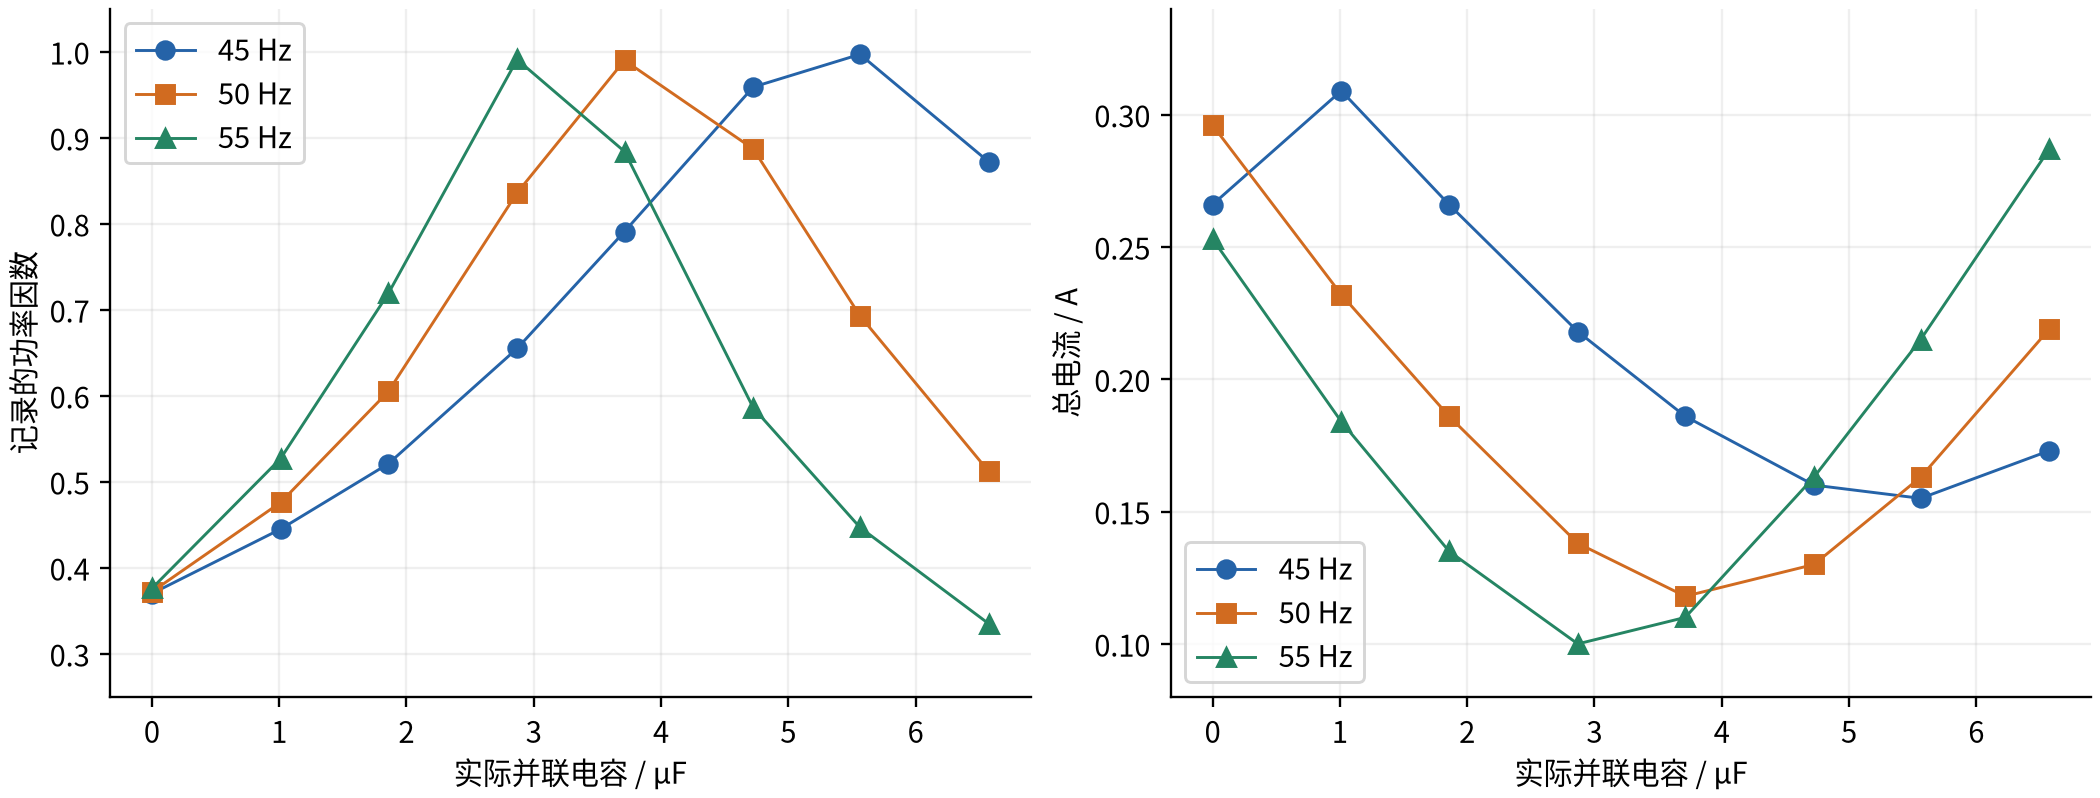
\includegraphics[width=\linewidth]{../assets/power_curves.png}\caption{功率因数与总电流随实际电容的变化}\end{figure}

三组功率因数均随电容增加先升高后降低，说明适当补偿有效，而过补偿会使效果变差。

接着，我用实测的 $P$、$U$、$I$ 核对功率因数。各组峰值处的对比如下。

\begin{center}\small
\begin{tabular}{cccc}
\toprule
频率/Hz & 档位 & 现场功率因数 & $P/(UI)$ \\
\midrule
45 & $C_6$ & 0.997 & 0.891 \\
50 & $C_4$ & 0.990 & 0.929 \\
55 & $C_3$ & 0.991 & 0.953 \\
\bottomrule\end{tabular}\end{center}

例如50 Hz、$C_4$处，$23.9/(218.1\times0.118)\approx0.929$。现场测量值与复算值存在差异，但峰值所在档位一致。下文仍按现场测量值比较，差异会在误差分析中讨论。

另外，同一频率下，有功功率变化较小：45 Hz为29.4—30.3 W，50 Hz为23.9—24.2 W，55 Hz为20.6—20.9 W。因此，并联电容主要改善功率因数、减小线路电流，并未明显降低负载的有功功率。

\clearpage

\subsection*{2. 最佳电容与有功功率}

依据上文的测量，按功率因数最大值选取最佳电容如下。

\begin{center}\small
\begin{tabular}{ccccc}
\toprule
频率/Hz & 最佳档位 & 实际电容/μF & 记录的最大功率因数 & 对应电流/A \\
\midrule
45 & $C_6$ & 5.5632 & 0.997 & 0.155 \\
50 & $C_4$ & 3.7135 & 0.990 & 0.118 \\
55 & $C_3$ & 2.8697 & 0.991 & 0.100 \\
\bottomrule\end{tabular}\end{center}

频率升高时，最佳档位对应的电容减小。由 $I_C=2\pi fCU$ 可知，同一电容的补偿电流随频率增大而增大。


\subsection*{4. 误差分析}

\begin{enumerate}
\item 标称1 μF的B号电容实测仅为0.6148 μF，说明标称值可能有较大偏差。因此，我在最终数据处理时，采用实测值计算组合电容，避免实验系统误差。
\item 实测电压为217.0—219.4 V。电源波动和灯管未稳定都可能影响读数，带来人为的读数误差。
\item 现场功率因数与 $P/(UI)$ 不完全一致，可能原因有未等到示数稳定就读数、仪表模式有误和仪表准确度较差。
\item 电容档位有限，峰值可能落在两档之间，可在最大值附近加密测量以获得更精确的最佳电容。

\end{enumerate}
各条件仅测一次，且缺少仪器允许误差限，因此本次不评定 A、B 类及合成标准不确定度。



